\documentclass{standalone}
\usepackage{pgfplots}
\pgfplotsset{compat=1.18}
\usepgfplotslibrary{fillbetween}
\usepackage{amsmath}

\begin{document}

\definecolor{tab_blue}{HTML}{1F77B4}
\definecolor{tab_orange}{HTML}{FF7F0E}
\definecolor{tab_green}{HTML}{2CA02C}
\definecolor{tab_red}{HTML}{D62728}

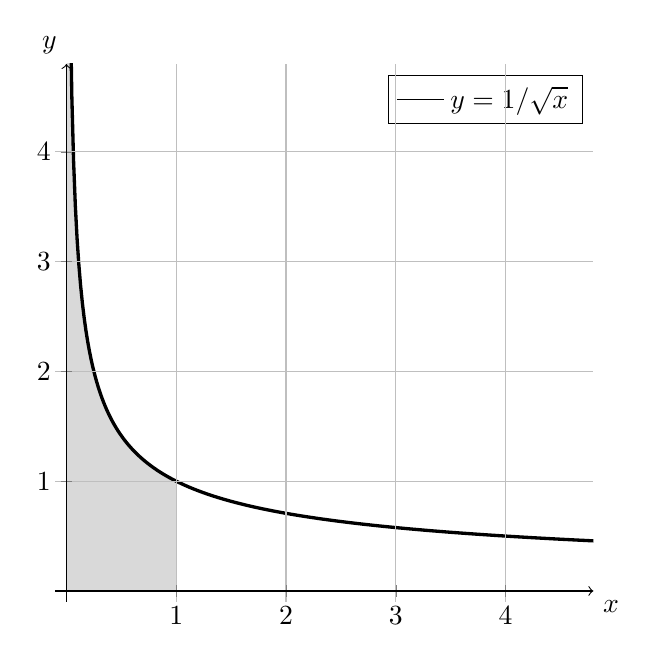
\begin{tikzpicture}[baseline]
\begin{axis}[
axis on top,
axis lines = middle,
unit vector ratio=1 1, 
% axis equal=false,
scale=1.2, 
xmin=-0.1, xmax=4.8, ymin=-0.1, ymax=4.8, 
grid = major,
xtick={0, 1, 2, 3, 4},
ytick={0, 1, 2, 3, 4},
xlabel=$x$,
ylabel=$y$,
xlabel style={below right},
ylabel style={above left},
axis line style = {->},
]

\addplot[samples=300, domain=0.001:1.0, name path=func] {1/(sqrt(x))};
\addplot[domain=0.001:1, name path=axis] {0}; 
\addplot[fill=gray!30] fill between [of=axis and func]; 
\addplot[samples=300, domain=0.001:4.8, very thick] {1/(sqrt(x))};
\legend{$y=1/\sqrt{x}$}
\end{axis}
\end{tikzpicture}

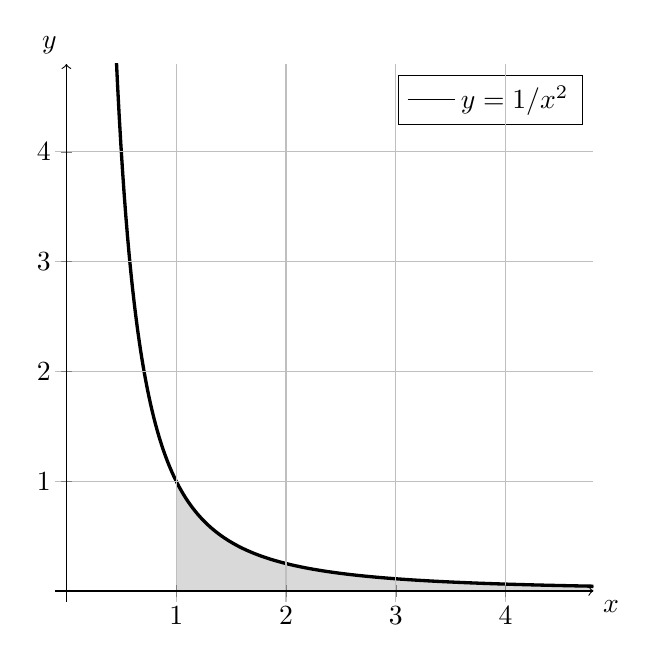
\begin{tikzpicture}[baseline]
\begin{axis}[
axis on top,
axis lines = middle,
unit vector ratio=1 1, 
% axis equal=false,
scale=1.2, 
xmin=-0.1, xmax=4.8, ymin=-0.1, ymax=4.8, 
grid = major,
xtick={0, 1, 2, 3, 4},
ytick={0, 1, 2, 3, 4},
xlabel=$x$,
ylabel=$y$,
xlabel style={below right},
ylabel style={above left},
axis line style = {->},
]

\addplot[samples=300, domain=1.0:4.8, name path=func] {1/x^2};
\addplot[domain=1.0:4.8, name path=axis] {0}; 
\addplot[fill=gray!30] fill between [of=axis and func]; 
\addplot[samples=300, domain=0.3:4.8, very thick] {1/x^2};
\legend{$y=1/x^2$}
\end{axis}
\end{tikzpicture}

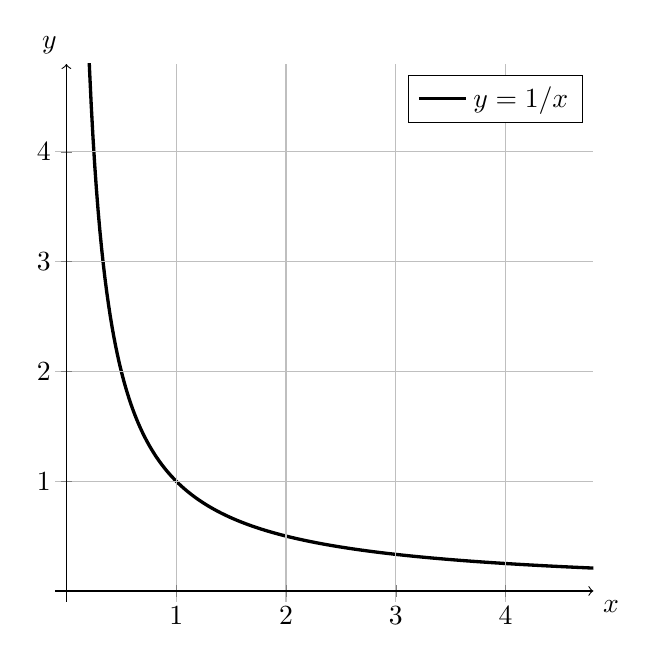
\begin{tikzpicture}[baseline]
\begin{axis}[
axis on top,
axis lines = middle,
unit vector ratio=1 1, 
% axis equal=false,
scale=1.2, 
xmin=-0.1, xmax=4.8, ymin=-0.1, ymax=4.8, 
grid = major,
xtick={0, 1, 2, 3, 4},
ytick={0, 1, 2, 3, 4},
xlabel=$x$,
ylabel=$y$,
xlabel style={below right},
ylabel style={above left},
axis line style = {->},
]

% \addplot[samples=300, domain=0.001:1.0, name path=func] {1/(sqrt(x))};
% \addplot[domain=0.001:1, name path=axis] {0}; 
% \addplot[fill=gray!30] fill between [of=axis and func]; 
\addplot[samples=300, domain=0.1:4.8, very thick] {1/x};
\legend{$y=1/x$}
\end{axis}
\end{tikzpicture}

\end{document}